\documentclass[11pt,a4paper]{article}
\usepackage[margin=25mm]{geometry}
\usepackage{amsmath,amssymb}
\usepackage{tikz}
\usepackage[hidelinks]{hyperref}
\setlength{\parindent}{0pt}
\setlength{\parskip}{6pt}
\newcommand{\code}[1]{\texttt{\detokenize{#1}}}

\title{Construction of the chopped spheroid source grid}
\author{Notes for the two-body Laplace experiments}
\date{15 September 2026}

\begin{document}
\maketitle

This note describes the construction actually implemented in the shared grid
builder and used by the sphere sweep:
\begin{quote}
\small
\code{laplace/lap3d_build_two_body_grids.m}\\
\code{sep15_sphere_laplace_spheroid_sweep.m}
\end{quote}
Each particle keeps its basic interior proxy sources and receives additional
sources on a chopped spheroid near contact.  The sweep uses spherical designs
for the sources.  For equal spheres, the dimensions now use the continuous
proxy radius, and the enhancing grid is mirrored between the particles.
The ellipsoid experiment retains its sampled-proxy enclosure rule.

\section{Axis, centre, and the requested tip}

Work with one particle at a time.  Its centre is $c$, its closest physical
contact point is $p$, and its accumulation points form a set $\mathcal A$.
Select
\[
 q=\underset{q_j\in\mathcal A}{\operatorname{argmin}}\,|q_j-p|,
 \qquad d=|q-c|,\qquad e=\frac{q-c}{d}.
\]
Thus $q$ is the accumulation point closest to the supplied contact point.
It is the point marked in black in the experiment figures.  Define
\[
 m=\frac{c+q}{2},\qquad f=\frac{d}{2}.
\]
The parent spheroid is centred at $m$ and its long axis is parallel to $e$.
Choose an orthogonal frame $U=[u_1,u_2,e]$ and write
$\xi=U^T(x-m)$.  Its surface and enclosed solid are respectively
\begin{equation}
 \frac{\xi_1^2+\xi_2^2}{B^2}+\frac{\xi_3^2}{A^2}=1,
 \qquad
 \frac{\xi_1^2+\xi_2^2}{B^2}+\frac{\xi_3^2}{A^2}<1,
 \label{eq:parent}
\end{equation}
where $A$ is the longitudinal semi-axis and $B$ is either transverse semi-axis.

Let $s=c+r_b e$ be the intersection of this outward radial line with the
physical boundary, and put $g=r_b-d$.  For an ellipsoid with body rotation $Q$
and semi-axes $a_1,a_2,a_3$,
\[
 r_b=\left(\sum_{i=1}^3\frac{(Q^Te)_i^2}{a_i^2}\right)^{-1/2}.
\]
For a sphere of radius $R$, $r_b=R$ and $g=|s-q|$ is also the shortest distance
from $q$ to the boundary.  For a general ellipsoid, $g$ is a \emph{radial}
distance, not necessarily the shortest Euclidean boundary distance; $s$ need
not equal $p$.

With requested parameter $0<\beta<1$, the initially requested semi-axis is
\begin{equation}
 A_0=f+\beta g.
 \label{eq:requested}
\end{equation}
If no further stretching is needed, the outward tip is
\[
 m+A_0e=q+\beta g e.
\]
It therefore lies a fraction $\beta$ of the way from $q$ towards $s$.
The opposite tip is $c-\beta g e$: stretching extends both ends because the
centre $m$ is fixed.

\section{Width rescaling and what ``confocal'' means}

The width parameter $w>0$ is set by \code{sourceWidthScale} in the grid options.
The sweep varies it through \code{widthScales}.  After choosing the final $A$,
the code sets
\begin{equation}
 B=w\sqrt{A^2-f^2}.
 \label{eq:width}
\end{equation}
At $w=1$, the foci are exactly $m\pm fe=c,q$, independently of $A$.
Consequently $c$ and $q$ are the \emph{foci}, not the tips of the final spheroid.
The limiting zero-width segment at $A=f$ has endpoints $c,q$.
Here ``confocal'' refers to this reference pair, not to the focal set of the
physical ellipsoid.

At fixed $A$, $w<1$ narrows the spheroid and $w>1$ widens it.  When $w\ne1$,
the actual focal half-length is
\[
 f_{\mathrm{actual}}=\sqrt{A^2-B^2},
\]
so the foci generally move away from $c,q$.  The code rejects $B>A$ because
that would produce an oblate rather than a prolate parent; $B=A$ is the
spherical limit.

\section{Sphere proxy radius, effective beta, and mirroring}

For spheres, let $\eta=\code{sourceOffset}$ and
$R_p=R-\eta$ be the radius of the basic proxy surface.  The reference point
is the intersection of that continuous sphere with the spheroid axis:
\[
 y_\rho=c+R_p e,\qquad U^T(y_\rho-m)=(0,0,R_p-f)^T.
\]
The implementation no longer searches for, or tries to enclose, the nearest
\emph{discrete} basic source.  Instead, the longitudinal semi-axis is
\begin{equation}
 A=\max\left\{f+\beta g,(1+10^{-10})|R_p-f|\right\},
 \qquad B=w\sqrt{A^2-f^2},\qquad
 \beta_{\mathrm{eff}}=\frac{A-f}{g}.
 \label{eq:effective}
\end{equation}
The small margin avoids an exactly tangent reference point when the radius
bound is active.  Since $A_0>f$, this radius bound is needed only when the
requested outward tip would fail to reach the proxy.  If it leaves only a
very small cap, a finite spherical design may contribute no retained sources;
increasing beta is then more useful than insisting on exact tangency.

Width rescaling does \emph{not} independently change the tip position or
effective beta for spheres.  Changing the basic source design or its node
count also does not change the parent dimensions.  In particular, for
$R=0.63$, $\delta=0.01$, and $\eta=0.125$, the accumulation point is already
outside the proxy radius, so $A=A_0$ and $\beta_{\mathrm{eff}}=\beta$ for all
the positive beta values in the sweep, up to roundoff.

Build and chop the first parent's design once.  To place it on the second
sphere, reflect its parent points and retained source points in the plane
halfway between the centres.  With
\[
 C=\frac{c_1+c_2}{2},\qquad
 \nu=\frac{c_2-c_1}{|c_2-c_1|},\qquad H=I-2\nu\nu^T,
\]
every enhancing point is mapped by
\begin{equation}
 y_{k,2}=C+H(y_{k,1}-C).
\end{equation}
Hence the two parents have the same semi-axes, the same effective beta, and
exactly mirrored cap nodes.  Both values are still recorded as
\code{effectiveBeta1} and \code{effectiveBeta2}, but they are now identical.
The existing basic source and collocation grids are unchanged; the whole
discrete linear system is therefore not being explicitly symmetrized.

The parent encloses $q$ and the axial continuous-proxy point $y_\rho$, and
therefore their connecting segment by convexity.  Enclosure of other sampled
basic proxy sources, or of an entire proxy patch, is neither required nor
claimed for this sphere construction.

\subsection{Ellipsoids: the existing sampled-proxy rule}

Let $Y_0$ be the \emph{discrete} basic source grid and select
\[
 y_* = \underset{y\in Y_0}{\operatorname{argmin}}\,|y-q|.
\]
Write $U^T(y_*-m)=(t_1,t_2,z)^T$ and
$v^2=(t_1^2+t_2^2)/w^2$.  To enclose $y_*$, equations
\eqref{eq:parent}--\eqref{eq:width} require
\[
 \frac{v^2}{A^2-f^2}+\frac{z^2}{A^2}<1.
\]
Setting $T=A^2$ and multiplying by the positive denominators gives
\[
 T^2-(f^2+z^2+v^2)T+z^2f^2>0.
\]
The relevant larger root is
\begin{equation}
 T_* = \frac{H+\sqrt{H^2-4z^2f^2}}{2},
 \qquad H=f^2+z^2+v^2.
\end{equation}
For ellipsoids, the unchanged choice, including a strict-enclosure margin, is
\begin{equation}
 A=\max\left\{A_0,(1+10^{-10})\sqrt{T_*}\right\},
 \qquad
 \beta_{\mathrm{eff}}=\frac{A-f}{g}.
\end{equation}
For this ellipsoid rule, narrowing the parent can also increase its length, so
requested and effective beta can differ.  In particular, sufficiently
small requested beta values can yield identical parents.  Effective beta is
recorded separately for the two bodies.

Since a spheroid encloses a convex solid, enclosing both $q$ and $y_*$ also
encloses their connecting line segment.  This is \emph{not} a guarantee of
enclosure of a whole proxy patch or every point between the accumulation set
and an entire proxy surface.  The current implementation uses the nearest
\emph{sampled} proxy point, not the nearest point on the continuous proxy.

\section{Discretization, chopping, and checks}

The function \code{get_sphdesign(Nreq)} loads the largest available design
with $N_{\mathrm{parent}}\le N_{\mathrm{req}}$ unit-sphere points
$\omega_k$.  These are mapped to the parent surface by
\begin{equation}
 y_k=m+U\,\operatorname{diag}(B,B,A)\,\omega_k.
\end{equation}
The design is spherical before this affine mapping; the mapped points do not
in general have equal physical-area spacing on the spheroid.

There are no independent cross-sectional and axial node counts for a
spherical design.  The existing alternative
\code{enhancingSourceDistribution = "tensor"} uses
\code{fineSourceResolution = [Nu,Nv]}: $N_u$ equally spaced azimuths on each
ring and $N_v$ Gauss--Legendre levels along the full parent axis.  The
parameterization before rotation and translation is
\[
 (B\sqrt{1-v^2}\cos u,\ B\sqrt{1-v^2}\sin u,\ Av),
 \qquad 0\le u<2\pi,\quad -1<v<1.
\]
Both counts are rounded to even integers.  The full tensor parent has
$N_uN_v$ nodes; the Gauss--Legendre levels cluster towards both tips without
including the tips themselves.  The \code{"quasiuniform"} alternative uses
the same axial levels but fewer azimuths on small rings.  These alternatives
are not spherical designs.  Chopping is applied after parent discretization
in every mode, so the retained cap count is smaller than the parent count.
The ellipsoid Laplace and Stokes entry points expose this resolution near
the top of the file.  Select tensor mode for a fixed count on every parent
ring, or quasiuniform mode for circumference-scaled counts near the tips.
In quasiuniform mode, \code{enhancingSourceExtraAzimuthNodes} raises the
counts on all rings, and \code{enhancingSourceMinAzimuthNodes} raises the
small-ring floor.  Their basic grids remain spherical designs; changing
\code{fineSourceResolution} does not alter those basic grids.  The sphere
entry points and sweep retain spherical-design defaults unless overridden.

The accuracy-check grid has its own controls:
\code{testResolution = [Nu,Nv]} sets the full-body repository quadrature,
while \code{testPatchLayers} and \code{testPatchAzimuthOversampling} set
additional near-contact evaluation rings.  Setting the test layer count to
zero disables those extra rings.  Evaluation rings use exponent
$\alpha+0.5$, outer angle $0.97\rho_{\max}$, and minimum azimuthal count
$n_{\min}+2$, distinct from the fitted collocation patch.  The contact point
itself is also checked.  Both the basic and enhanced solutions are evaluated
on exactly the same test nodes, which never enter their least-squares
matrices.  Refining the test grid can increase the measured maximum residual
by revealing previously unsampled peaks; it does not change the fitted
solution.  Increase the evaluation controls until the maximum stabilizes.

Let $\eta=\code{sourceOffset}$,
$\zeta=\code{sourceChopOffset}$, and let
$\operatorname{dist}(y,\partial\Omega)$ be the shortest distance to the
physical boundary.  The chopped cap consists of parent nodes satisfying
\begin{equation}
 0<\operatorname{dist}(y_k,\partial\Omega)<\eta+\zeta,
 \qquad \eta+\zeta>0.
 \label{eq:chop}
\end{equation}
The default $\zeta=0$ removes points deeper inside the basic proxy and keeps
the shallow, contact-facing portion.  Positive $\zeta$ extends the retained
cap deeper into the proxy; negative $\zeta$ stops the cap short of the proxy.
This signed offset is in physical length units and changes only the cut,
not the parent axes or the beta-controlled contact-facing tip.  The cut is
not generally a plane.  Finite sampling may leave the last retained node
short of the intended cut; increasing the design count or the tensor axial
resolution resolves that edge more closely.
For a sphere, the basic proxy is the concentric sphere of radius $R-\eta$,
so the retained-node test is exactly
\[
 R-\eta-\zeta<|y_k-c|<R.
\]
For an ellipsoid, chopping uses distance to the physical boundary and the
normal-offset depth; it does not fit a confocal ellipsoid to the basic nodes.
If \code{removeDuplicates} is true, near-duplicates against the basic grid
and other accepted cap points are then removed with tolerance
$10^{-11}\max_i a_i$.  Setting it false preserves all retained source nodes;
collocation deduplication is unchanged.  Overlap with the proxy can make
source columns more redundant, so compare maximum residuals and coefficient
magnitudes when increasing $\zeta$.

\begin{figure}[ht]
\centering
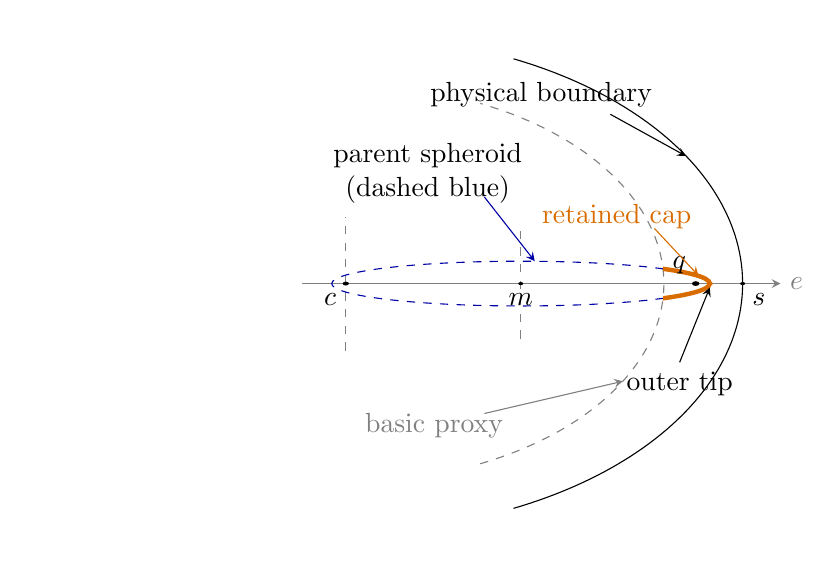
\begin{tikzpicture}[x=8cm,y=5cm,>=stealth]
 \def\R{0.63}
 \def\proxy{0.505}
 \def\midpoint{0.2777350657}
 \def\longaxis{0.3000940263}
 \def\shortaxis{0.0568323365}
 \draw[gray,dashed] (0,-0.17)--(0,0.17);
 \draw[gray,dashed] (\midpoint,-0.14)--(\midpoint,0.14);
 \draw[->,gray] (-0.07,0)--(0.69,0) node[right] {$e$};
 \draw[black] plot[domain=-65:65,samples=100]
   ({\R*cos(\x)},{\R*sin(\x)});
 \draw[gray,dashed] plot[domain=-65:65,samples=100]
   ({\proxy*cos(\x)},{\proxy*sin(\x)});
 \draw[blue!65!black,dashed]
   (\midpoint,0) ellipse[x radius=\longaxis,y radius=\shortaxis];
 \begin{scope}[even odd rule]
   \clip (-0.08,-0.65) rectangle (0.72,0.65)
      (0,0) circle (\proxy);
   \draw[orange!85!black,line width=1.6pt]
      (\midpoint,0) ellipse[x radius=\longaxis,y radius=\shortaxis];
 \end{scope}
 \fill (0,0) circle[radius=0.005] node[below left] {$c$};
 \fill (\midpoint,0) circle[radius=0.004] node[below] {$m$};
 \fill (0.5554701314,0) circle[radius=0.006];
 \node[above left] at (0.5554701314,0) {$q$};
 \fill[orange!85!black] (0.577829092,0) circle[radius=0.005];
 \draw[->] (0.53,-0.20)--(0.577829092,-0.01);
 \node[below] at (0.53,-0.20) {outer tip};
 \fill (\R,0) circle[radius=0.004] node[below right] {$s$};
 \node[align=center] at (0.13,0.28) {parent spheroid\\(dashed blue)};
 \draw[->,blue!65!black] (0.22,0.22)--(0.30,\shortaxis);
 \node[gray] at (0.14,-0.36) {basic proxy};
 \draw[->,gray] (0.22,-0.33)--(0.44,-0.248);
 \node at (0.31,0.48) {physical boundary};
 \draw[->] (0.42,0.43)--(0.54,0.324);
 \node[orange!85!black] at (0.43,0.17) {retained cap};
 \draw[->,orange!85!black] (0.49,0.14)--(0.56,0.020);
\end{tikzpicture}
\caption{Meridional cross-section for one sphere, $R=0.63$, $\delta=0.01$,
 $\eta=0.125$, $\beta_{\mathrm{eff}}=0.3$, and $w=0.5$.
 Only the contact-facing portion of the physical boundary and proxy is drawn.
 Vertical and horizontal scales differ for readability.
 The orange curve is a portion of the same parent spheroid, not a second
 surface and not a planar lid closing the chopped surface.}
\end{figure}

The code checks that all supplied accumulation points lie strictly inside
both their physical body and the parent spheroid, and that every discretized
parent point is inside the body.  Ellipsoids additionally require enclosure
of their sampled proxy point $y_*$.  Spheres do not require that test.  A failed
accumulation-enclosure check causes an error; it does not automatically
enlarge the parent for every accumulation point.  Retained sources are checked
again for physical interiority.  For spheres, $|m-c|+A<R$ additionally checks
containment of the whole continuous prolate parent: its outer tip is the point
of greatest distance to the body centre.  For ellipsoids, the physical
containment test remains a check at the discretized parent points, not an
analytic proof for the entire continuous parent surface.

\section{The meaning of \code{cap1/cap2}}

The printed column \code{cap1/cap2} means
\[
 \underbrace{N_{\mathrm{cap},1}}_{\text{enhancing sources on particle 1}}
 \quad/\quad
 \underbrace{N_{\mathrm{cap},2}}_{\text{enhancing sources on particle 2}},
\]
\emph{after chopping and duplicate removal}.  These are not collocation-node
counts, coefficient magnitudes, the two tips of one spheroid, or a comparison
between two source shapes.  There is one chopped parent per particle.
For example, \code{20/20} means twenty additional sources on each particle.
The printed slash separates two integer counts; it is not a quotient.

The corresponding sweep columns are \code{capNodes1} and \code{capNodes2}.
If $N_{0,i}$ denotes the basic source count, the total number of physical
source locations (also the monopole-only unknown count) is
\[
 N_{\mathrm{total}}=N_{0,1}+N_{\mathrm{cap},1}
                  +N_{0,2}+N_{\mathrm{cap},2}.
\]
The collocation patch is generated independently by
\code{lap3d_collocation_patch.m}; it is not counted in \code{cap1/cap2}.
The separate \code{capCoefficientInf} column is the maximum absolute
coefficient over the enhancing sources on \emph{both} particles.

For equal spheres, the first cap is chopped and deduplicated, then mirrored
without an independent second cut.  Thus the cap counts are now identical.
For ellipsoids, the two independently constructed caps can still have
different counts and effective beta values.

\section{Enhancing Laplace basis: monopoles or SLP plus DLP}

Each Laplace grid experiment exposes
\code{gridControls.enhancingLaplaceBasis = "SLP"} near the top.
This is the default monopole-only representation.  Set it to
\code{"SLP+DLP"} to add one independently fitted normal dipole at every
retained enhancing node.  Basic proxy nodes remain monopole-only, and this
switch changes neither source locations nor collocation/evaluation grids.
It applies equally to chopped spheroids, both comparison sphere caps,
the node/beta/width sweep, and the randomized ellipsoid experiment.

With $r=x-y$, the two point-source kernels are
\[
 G(x,y)=\frac{1}{4\pi|r|},\qquad
 H(x,y)=\partial_{n_y}G(x,y)
       =\frac{n_y\cdot r}{4\pi|r|^3}.
\]
Here $n_y$ is the outward unit normal of the \emph{parent source surface},
not the normal of the physical body or a cut-plane normal.  If the parent's
centre is $m$, rotation is $Q$, and semiaxes are $s$, this direction is
\[
 n_y=\frac{A_p(y-m)}{|A_p(y-m)|},\qquad
 A_p=Q\,\operatorname{diag}(s_1^{-2},s_2^{-2},s_3^{-2})Q^{\mathsf T}.
\]
These are discrete MFS strengths, not layer densities with quadrature
weights.  Targets lie on the physical body, away from the interior source
surface, so no boundary jump term is included.

The positive physical length
\code{gridControls.laplaceDipoleLengthScale = 1} multiplies the DLP columns:
\[
 u(x)=\sum_{j=1}^{N_{\mathrm{total}}}q_jG(x,y_j)
       +L\sum_{j\in\mathrm{cap}}d_jH(x,y_j).
\]
Thus $q_j$ and the \emph{fitted} $d_j$ have common charge units; the physical
dipole moment is $L d_jn_j$.  Keep $L$ fixed when comparing coefficient
maxima.  Changing it is a basis scaling that can affect a truncated-SVD
solution, not a physical reduction of source strength.  The coefficient
vector order is all body-ordered monopoles, followed by cap-node dipoles.
These coefficients are independent; there is no prescribed coupling ratio.

In combined mode the number of unknowns is
\[
 N_{\mathrm{unknown}}=N_{\mathrm{total}}
             +N_{\mathrm{cap},1}+N_{\mathrm{cap},2}.
\]
\code{cap1/cap2} still counts physical enhancing locations, not coefficients.
The sweep reports these quantities separately as \code{totalSources},
\code{totalUnknowns}, and \code{dipoleUnknowns}.  Matrix previews include the
extra DLP columns; the collocation count must exceed the full unknown count.
Each body's charge sums only its $q_j$: dipoles have zero net charge.
Reported coefficient maxima include both fitted families.  Source scatter
colors show $\log_{10}\max(|q_j|,|d_j|)$ at each physical location, using
$d_j=0$ on the basic proxy and separate color scales for every panel.
Previously reported numerical examples below used \code{"SLP"} only.

\section{Optional column scaling and surface-element preconditioning}

Two independent booleans near the top of each Laplace grid experiment are:
\begin{quote}
\small
\code{gridControls.columnScaling}\\
\code{gridControls.surfaceElementPreconditioning}
\end{quote}
Both default to
\code{false}, preserving the previous unscaled solve. They apply to both
basic and enhanced systems, including both comparison sphere caps and all
sweep or randomized configurations. They change no node locations.

Let $A$ be the physical MFS matrix, $b$ the prescribed boundary data, and
$w_i>0$ the local physical surface area represented by collocation node $i$.
When surface-element preconditioning is enabled, define
\[
 W_{ii}=\sqrt{w_i};
\]
otherwise $W=I$. Multiply \emph{both} the equations and their data by $W$.
After this row weighting, enabled column scaling sets
\[
 C_{jj}=\frac{1}{\|(WA)_{:,j}\|_2};
\]
otherwise $C=I$. The numerical solve is
\[
 B=WAC,\qquad g=Wb,\qquad z=B^+_{\tau}g,\qquad c=Cz,
\]
where $B^+_{\tau}$ is the truncated-SVD pseudoinverse using the selected
relative cutoff $\tau$. Returned coefficients $c$, charges, dipole moments,
and source-magnitude plots are all in the original physical units: the
column scaling is \emph{undone}, not presented as smaller physical strengths.
The singular values, retained rank, and retained condition number now refer
to $B$, not $A$. Thus a fixed cutoff can select different modes when either
preconditioner is changed. Column normalization uses a 2-norm internally;
all reported residual and coefficient maxima remain infinity norms.

The shared function \code{lap3d_collocation_surface_elements} estimates
$w_i$ on each \emph{complete merged} collocation grid. It maps the physical
nodes to the unit parameter sphere, triangulates them, and shares each
spherical triangle's solid angle equally between its three vertices. If
the resulting angular area at direction $u_i$ is $\Omega_i$, then
\[
 w_i=\Omega_i J(u_i),\qquad
 J(u)=a_1a_2a_3\sqrt{\sum_{k=1}^3u_k^2/a_k^2}.
\]
These are positive lumped local-area estimates, not the original high-order
quadrature weights. For spheres, $J=R^2$ and the total is exactly $4\pi R^2$
up to roundoff. For ellipsoids the total physical area is approximated.
Recomputing after merging the patch avoids counting its overlap with the
basic grid twice and assigns smaller area per node in densely sampled regions.

Without truncation, row weighting fits $\sum_iw_i|(Ac-b)_i|^2$, an
approximation to the integrated squared surface residual, not its maximum.
This can reduce the influence of a densely sampled contact patch compared
with unweighted least squares; it does \emph{not} guarantee a lower maximum
contact residual or smaller physical coefficients. Both collocation and
independent evaluation residuals are recomputed with the physical kernels
and remain unweighted: $\|Ac-b\|_\infty/\|b_{\mathrm{body}}\|_\infty$.
The solution stores \code{rowScalingFactors}, \code{columnScalingFactors},
and \code{scaledCoefficients} so that the numerical transformation is explicit.

\section{Basic collocation counts and approval before solving}

In \code{basicGridDistribution = "sphericaldesign"} mode,
\code{basicSourceCount} and \code{basicCollocationCount} request the numbers
per particle.  Each request loads the largest available design not exceeding
the requested count, so the actual count need not equal the requested one.
In \code{"ellipsoidquadrature"} mode, these design counts are ignored.
\code{coarseSourceResolution = [Nu,Nv]} instead controls the original source
quadrature.  The optional \code{basicCollocationResolution = [Nu,Nv]} sets
the physical boundary quadrature independently, without changing any source
nodes.  Leaving it \code{[]} preserves the current repository oversampling.
All quadrature counts are whole-surface counts before the two-body mapping;
the actual number is the sum of the variable azimuthal counts on the
Gauss--Legendre rings, not necessarily $N_uN_v$.

The experiment default \code{confirmBeforeSolve = true} builds geometry and
grids to obtain exact dimensions, then reports the basic and enhanced system
sizes and the memory for each dense matrix alone.  Stokes dimensions include
three velocity components and three unknowns per selected enhancing family
per node.  Kernel temporaries, SVD factors and workspace require additional
memory.  No kernel assembly, SVD solve or solution evaluation starts until
the user enters \code{y} or \code{yes}.  Other answers, including empty or
unavailable input, cancel and return an empty result.  Setting the flag false
is an explicit bypass for an already-approved automated run.

\section{Enhancing collocation counts and patch refinement}

The enhancing collocation nodes are generated separately on the physical
surface, not on the spheroid.  The controls used below are:
\begin{center}
\begin{tabular}{ll}
 $L$ & \code{collocationPatchLayers}\\
 $\alpha$ & \code{collocationExponent}\\
 $\rho_{\max}$ & \code{collocationPatchAngle}\\
 $n_{\min}$ & \code{collocationMinAzimuth}\\
 $\chi$ & \code{collocationAzimuthOversampling}
\end{tabular}
\end{center}
The ring radii and radial spacings on the parameter sphere are
\[
 \rho_j=\rho_{\max}\frac{\exp(\alpha j/L)-1}{\exp(\alpha)-1},
 \qquad \Delta\rho_j=\rho_j-\rho_{j-1},\quad \rho_0=0.
\]
The azimuthal count $n_j$ is
\[
 n_j=\operatorname{evenceil}\left[
  \max\left\{n_{\min},
  \left\lceil\chi\frac{2\pi\sin\rho_j}{\Delta\rho_j}\right\rceil\right\}
 \right],
\]
where $\operatorname{evenceil}$ rounds upwards to an even integer.
There is also one contact node per particle.  The generated count per patch
is $1+\sum_j n_j$.  The reported
\code{totalEnhancingCollocation} is the sum of the \emph{retained} patch
counts on both particles after removing duplicates against the basic grid.
It excludes basic collocation points and independent evaluation points.
The per-particle sweep columns are \code{enhancingCollocation1} and
\code{enhancingCollocation2}; \code{totalCollocation} includes both basic
and enhancing collocation points.

For $\rho_{\max}=0.5$, $\alpha=3$, and $n_{\min}=8$, these sphere grids give:
\begin{center}
\begin{tabular}{rrrr}
 $L$ & $\chi$ & patch points per particle & enhancing total\\\hline
 18 & 1 & 535 & 1070\\
 36 & 1 & 1987 & 3974\\
 36 & 2 & 3939 & 7878
\end{tabular}
\end{center}

Increase $L$ first to decrease radial spacing; this also increases the
circumference-based azimuthal counts.  Increase $\chi$ to refine all rings
azimuthally, or increase $n_{\min}$ to refine only the rings constrained by
that floor.  Increase $\alpha$ only when residual peaks are concentrated very
near contact: it redistributes the rings inward but makes outer spacing
coarser at fixed $L$.  Reduce $\rho_{\max}$ only if the whole problematic
region remains covered; increase it when residual peaks reach the patch edge.

More collocation points do not guarantee a smaller maximum residual.  The
truncated SVD solves a discrete least-squares problem, not a minimax problem;
changing sampling density changes the relative emphasis on different regions.
For a fixed source basis, a residual can plateau because it cannot represent
the boundary data more accurately.  Compare refinements on the \emph{same}
independent evaluation grid, including finer contact rings, while keeping
source points and the SVD cutoff fixed.

In a helper regression at $R=0.63$, $\delta=0.01$, $\beta=0.3$, $w=0.5$,
700 requested basic sources, and 640 requested parent nodes, increasing
$L$ from 18 to 36 reduced the independent max residual from approximately
$2.14\times10^{-5}$ to $2.01\times10^{-5}$.  Setting $\chi=2$ then gave
$2.33\times10^{-5}$, rather than further improvement.  With only 200 requested
parent nodes, radial refinement instead left the residual near
$1.5\times10^{-4}$.  These checks illustrate the source-basis limitation and
the sampling/least-squares tradeoff; they do not establish a universal
refinement rate.

\section{Sphere specialization and a concrete example}

For equal spheres of radius $R$ and surface gap $\delta$, the shared geometry
places their centres at $\pm(R+\delta/2)e_x$.  Their accumulation points are
\[
 q_1=-h e_x,\qquad q_2=h e_x,\qquad
 h=\frac{\sqrt{\delta(4R+\delta)}}{2}.
\]
The stored accumulation arrays repeat these points over the angular samples;
they are not distinct lines or rings for spheres.  On either body,
\[
 d=R+\delta/2-h,\qquad f=d/2,\qquad g=h-\delta/2.
\]
For the verified setup with $R=0.63$, $\delta=0.01$, $\beta=0.3$, $w=0.5$,
and no additional proxy-enclosure stretching,
\[
 f\simeq0.2777351,\qquad g\simeq0.0745299,\qquad
 A\simeq0.3000940,\qquad B\simeq0.0568323.
\]
In that run, a request for $200$ enhancing nodes loads a $182$-point parent
design and leaves \code{cap1/cap2 = 20/20}.  The basic requests
$1000/1600$ sources/collocation per particle give actual basic counts
$969/1569$.  With 24 collocation patch layers, potentials $[1;-1]$, and SVD
cutoff $10^{-13}$, the mirrored-grid helper check gave a coefficient max norm
of about $0.848$ and an independent boundary residual max norm of about
$7.24\times10^{-5}$, checked at 27,104 evaluation points.
Its enhancing collocation count was $921+921=1842$.
These are numerical results for that setup, not a geometric bound or a
guarantee for other resolutions, gaps, widths, or beta values.

\end{document}
